\documentclass[
    11pt,
    preprint,
    author-numerical,
    aps,
    prl, % Physical Review A, the default.
    natbib,
    superscriptaddress,
]{revtex4-2}

\setcitestyle{authoryear}

\RequirePackage{luatex85, shellesc} % work around the LuaTex bug
% options for packages which may be loaded elsewhere
\PassOptionsToPackage{unicode=true, pdfa}{hyperref}
\PassOptionsToPackage{hyphens}{url}
\PassOptionsToPackage{dvipsnames,svgnames*,x11names*}{xcolor}

%==============================================================================%
%                                Load packages                                 %
%==============================================================================%

\usepackage{amsmath}     % the AMS Math package - provides useful math environments and tools

\usepackage{amssymb}     % provides useful symbols

\usepackage{amsfonts}    % provides nice mathematical fonts

\usepackage{bm}          % bold math

\usepackage{calc}        % gives the ability to calculate in the document itself, inferior to but lighter weight than pythontex

\usepackage{cancel}      % provides environments to cancel stuff in mathmode

\usepackage{dcolumn}     % Align columns on decimal point

\usepackage{esint}       % better and more integral signs

\usepackage{enumitem}    % enumerate and itemize improvements

\usepackage{fancyhdr}    % fancy headers and footers

\usepackage{fancyref}    % for fancy cross-referencing with vario-style refs

\usepackage{graphicx}    % facilitates inclusion of external graphics

\usepackage{microtype}   % typographical improvements, kerning, etc

\usepackage{parskip}     % produces zero \parindent and non-zero \parskip

\usepackage{setspace}    % set space between lines

\usepackage{siunitx}     % for the use of SI unite in mathmode

\usepackage{xcolor}      % colours bro

\usepackage{upquote}     % straight quotes in verbatim environments

\usepackage{unicode-math} % allows unicode characters in mathmode

\usepackage[pdfa, unicode]{hyperref} % hyperlinks and PDF metadata manipulation

\usepackage{tikz}        % drawing

\usepackage{pgfplots}    % plotting

\usepackage{geometry}    % to set the margins of the page

%==============================================================================%
%                             Set package options                              %
%==============================================================================%

%============================%
%          AMSMath           %
%============================%

\allowdisplaybreaks

%============================%
%          Hyperref          %
%============================%

\hypersetup{
    pdftitle={A minimal reaction-diffusion neural model generates C. elegans undulation},
    pdfauthor={Anshul Singhvi},
    colorlinks=true,
    linkcolor=Maroon,
    citecolor=Blue,
    urlcolor=Blue,
    breaklinks=true,
    pdfdisplaydoctitle = true
}

%============================%
%         Microtype          %
%============================%

\UseMicrotypeSet[protrusion]{basicmath} % disable protrusion for tt fonts

%============================%
%     TikZ and PGFPlots      %
%============================%

\usetikzlibrary{
    arrows.meta,
    calc,
    decorations,
    decorations.pathreplacing,
    decorations.footprints,
    math,
    patterns,
    shadows,
    external
}

\tikzset{>=stealth}

\pgfplotsset{compat=1.16}

\usepgfplotslibrary{
    polar,
    colormaps,
    colorbrewer,
    groupplots,
    statistics
}

% This cycle list encodes the Wong colors, which are visually distinguishable.
% They also account for colorblind support, and as such are optimal for use in a paper.
\pgfplotscreateplotcyclelist{wong}{%
    color={rgb, 255 : red, 86  ; green, 180 ; blue, 233}, mark = *\\         % sky blue
    color={rgb, 255 : red, 230 ; green, 159 ; blue, 0},   mark = square*\\   % orange
    color={rgb, 255 : red, 0   ; green, 158 ; blue, 115}, mark = otimes*\\   % blueish green
    color={rgb, 255 : red, 240 ; green, 228 ; blue, 66},  mark = star\\      % yellow
    color={rgb, 255 : red, 0   ; green, 114 ; blue, 178}, mark = diamond*\\  % blue
    color={rgb, 255 : red, 213 ; green, 94  ; blue, 0},   mark = triangle*\\ % vermillion
    color={rgb, 255 : red, 204 ; green, 121 ; blue, 167}, mark = pentagon*\\ % reddish purple
}

\pgfplotsset{every axis legend/.append style={%
        cells={anchor=west}
    },
    cycle list name = wong,
}

%============================%
%          Geometry          %
%============================%

\geometry{
  a4paper,
  margin = 1.2in
}

%==============================================================================%
%                         Macros and document options                          %
%==============================================================================%

\setstretch{1} % line spacing of 1.25

\setlength{\emergencystretch}{3em}  % prevent overfull lines
\providecommand{\tightlist}{%
  \setlength{\itemsep}{0pt}\setlength{\parskip}{0pt}}
% \setcounter{secnumdepth}{0}
%
% % Redefines (sub)paragraphs to behave more like sections
% \ifx\paragraph\undefined\else
%     \let\oldparagraph\paragraph
%     \renewcommand{\paragraph}[1]{\oldparagraph{#1}\mbox{}}
% \fi
% \ifx\subparagraph\undefined\else
%     \let\oldsubparagraph\subparagraph
%     \renewcommand{\subparagraph}[1]{\oldsubparagraph{#1}\mbox{}}
% \fi

\newcommand{\inputtikz}[1]{%
  \tikzsetnextfilename{#1}%
  \input{#1.tikz}%
}

%==============================================================================%
%                            Neuron diagram macros                             %
%==============================================================================%

\newcommand{\doublec}[2]{% double diffusion arrows
  \draw  [-Circle] ($(#1.north east)!0.7!(#1.north)$) -- ($(#2.south east)!0.7!(#2.south)$);
  \draw  [Circle-] ($(#1.north west)!0.7!(#1.north)$) -- ($(#2.south west)!0.7!(#2.south)$);
  }

\newcommand{\singlec}[2]{% single diffusion arrows
  \draw [-Latex] (#1.east) -- (#2.west);
  }


\tikzexternalize

\begin{document}

%==============================================================================%
%                              Title and abstract                              %
%==============================================================================%

\title{A minimal reaction-diffusion neural model generates {\emph{C. elegans}} undulation}
\author{Anshul Singhvi}
\affiliation{Bard College at Simon's Rock}
\author{Harold Hastings}
\affiliation{Bard College at Simon's Rock}
\affiliation{Hofstra University}
\author{Jennifer Magnes}
\affiliation{Vassar College}
\author{Cheris Congo}
\affiliation{Vassar College}
\author{Miranda Hulsey-Vincent}
\affiliation{Vassar College}
\author{Rifah Tasnim}
\affiliation{Bard College at Simon's Rock}
\author{Naol Negassa}
\affiliation{Bard College at Simon's Rock}
\date{\today}
\begin{abstract}
    The small (1 mm) nematode \emph{Caenorhabditis elegans} has become widely used as a model organism; in particular the \emph{C. elegans} connectome has been completely mapped, and \emph{C. elegans} locomotion has been widely studied (c.f. http://www.wormbook.org \citep{corsi2015}). We describe a minimal reaction-diffusion model for the \emph{C. elegans} central pattern generator (CPG) \citep{xu2018,wen2012}. We use simulation methods to show that a small network of \cite{fitzhugh1955}-\cite{nagumo1962} neurons (one of the simplest neuronal models) can generate key features of \emph{C. elegans} undulation \citep[see][]{magnes2012} and thus locomotion. Compare the neuromechanical model of \cite{izquierdo2018}. We also investigate dynamics and stability of the model.
\end{abstract}

\maketitle

\section{Introduction}\label{sec: intro}

The small (1 mm) nematode \emph{Caenorhabditis elegans} (\emph{C. elegans}) has become widely used as a model organism \citep{corsi2015}, and has been among the most widely studied biological models of neuronal development, locomotion and the central pattern generator \citep{katz2016}.
The C. elegans connectome has been completely mapped \citep{jabr} and, as described below, its locomotion has been widely studied.
``When crawling on a solid surface, the nematode C. elegans moves forward by propagating sinusoidal dorso-ventral retrograde contraction waves. A uniform propagating wave leads to motion that undulates about a straight line.'' \citep{kim2011}.
A different type of locomotion, often called swimming, occurs when nematodes are submerged in a liquid medium. The nematodes “switch” between these two gaits, under the regulation of particular serotonergic and dopaminergic neurons.

The purpose of this paper to describe a minimal reaction-diffusion model for the C. elegans central pattern generator (CPG) \citep{xu2018, wen2012}. We use simulation methods to show that a small network of \cite{fitzhugh1955}-\cite{nagumo1962} neurons (one of the simplest neuronal models) based on a skeleton model of the C. elegans CPG can reproduce key features of C. elegans undulation \citep{magnes2012} and thus locomotion.

\section{The model central pattern generator}

The central pattern generator is a small neural circuit which regulates the movement of the nematode.  This structure is present in different forms in many different animals, and it regulates many different types of regular movement.

\begin{figure}[h!]
    \label{fig: xu_cpg}
    \centering
    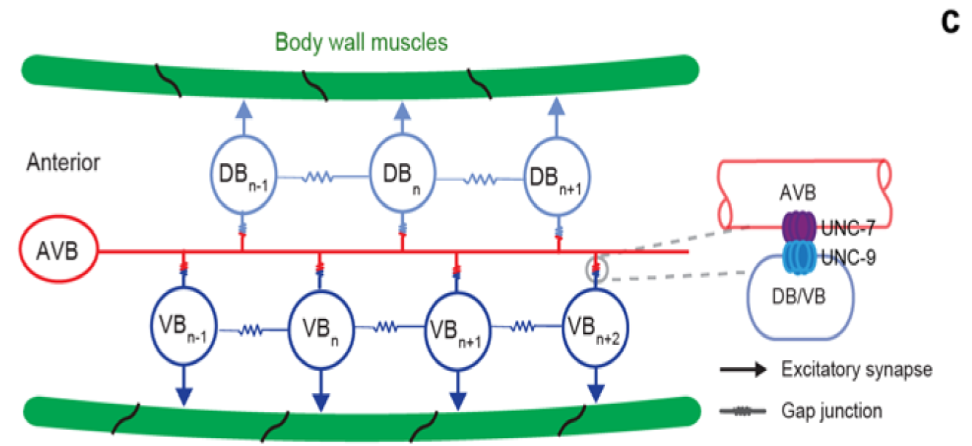
\includegraphics[width=7cm]{figures/xu_cpg/xu_cpg.png}
    \caption{Pirated from Xu}
\end{figure}


% \inputtikz{figures/fhn_dynamics/fhn_dynamics}


\section{Correspondence}\label{correspondence}
\makeatletter
Please direct all correspondence to hhastings@simons-rock.edu,
jemagnes@vassar.edu, or\\asinghvi17@simons-rock.edu.
\makeatother

\section{References}

\nocite{*}
\bibliography{References}
% \printbibliography[heading=none]
\end{document}
